%
% Komplexe Differenzierbarkeit
%
\subsection{Komplexe Differenzierbarkeit
\label{buch:holomoprh:holomorph:subsection:komplexedifferenzierbarkeit}}
Im Anfängerunterricht der Analysis wird meistens der Begriff der Steigung
einer Tangente an den Graphen einer Funktion als Motivation für die Definition
der Ableitung der Funktion verwendet.
Diese geometrische Intuition funktioniert für komplexe Funktionen
nicht mehr, da der Graph einer komplexen Funktion eine Fläche in einem
vierdimensionalen reellen Vektorraum ist, der unserer Anschauung unzugänglich
ist.
Es muss daher eine rein analytische Definition gefunden werden.

%
% Ableitungen als Differenzenquotienten
%
\subsubsection{Ableitungen als Differenzenquotienten}
Die Ableitung einer reellen Funktion $f\colon I \to\mathbb{R}$ wird oft
als der Grenzwert 
\[
f'(x) = \lim_{h\to 0} \frac{f(x+h) - f(x)}{h}
\]
eingeführt.
Eine komplexe Funktion können wir als zwei reellwerte Funktionen
von \emph{zwei} reellen Variablen $x$ und $y$ betrachten, es gibt
daher die vier verschiedene reelle Ableitungen
\begin{align*}
\frac{\partial u}{\partial x}(x,y)
&=
\lim_{h\to0} \frac{u(x+h,y)-u(x,y)}{h},
&
\frac{\partial v}{\partial x}(x,y)
&=
\lim_{h\to0} \frac{v(x+h,y)-v(x,y)}{h},
\\
\frac{\partial u}{\partial y}(x,y)
&=
\lim_{h\to0} \frac{u(x,y+h)-u(x,y)}{h},
&
\frac{\partial v}{\partial y}(x,y)
&=
\lim_{h\to0} \frac{v(x,y+h)-v(x,y)}{h}.
\end{align*}
Zusammen bilden diese Ableitungen die Jacobi-Matrix
\index{Jacobi-Matrix}%
\[
\Jf(x,y)
=
\frac{\partial (u,v)}{\partial(x,y)}
=
\renewcommand{\arraystretch}{1.8}
\begin{pmatrix}
\displaystyle \frac{\partial u}{\partial x}(x,y)
&
\displaystyle \frac{\partial u}{\partial y}(x,y)
\\
\displaystyle \frac{\partial v}{\partial x}(x,y)
&
\displaystyle \frac{\partial v}{\partial y}(x,y)
\end{pmatrix}.
\]
Welche dieser partiellen Ableitungen kann die Rolle einer komplexen
Ableitung übernehmen?
Offenbar reicht die Idee des Differenzenquotienten allein nicht aus,
um eine komplexe Ableitung zu definieren.

%
% Die lineare Ersatzfunktion
%
\subsubsection{Die lineare Ersatzfunktion}
Die Ableitung kann aber auch als eine lineare Approximation
der Funktion betrachtet werden.
Für eine Funktion einer Variablen ist die Taylor-Reihe
\index{Taylor-Reihe}%
\[
f(x+h)
=
f(x)
+
f'(x) h
+
\frac{f''(x)}{2!}h^2
+
\dots
.
\]
Die Terme mindestens quadratischer Ordnung in $h$ können zusammengefasst
werden in einen Ausdruck $o(h)$ mit der Eigenschaft, dass
\[
\lim_{h\to 0}
\frac{o(h)}{h}
\]
ist.
Damit lässt sich die Taylor-Reihe schreiben als
\[
f(x+h)
=
f(x) + f'(x) h + o(h).
\]
Die ersten zwei Terme bilden eine lineare Funktion, die bis auf
die Korrektur $o(h)$ kleinerer Ordnung die Funktion $f(x+h)$
korrekt wiedergibt.
Solange man also nur eine lineare Approximation benötigt, ist
\begin{equation}
f(x+h)
\approx
f(x) + f'(x) \cdot h
\label{buch:holomorph:holomorph:1dersatz}
\end{equation}
die geeignete \emph{lineare Ersatzfunktion}.
\index{lineare Ersatzfunktion}%

Die Taylor-Reihe der als Abbildung $\mathbb{R}^2\to\mathbb{R}^2$
betrachteten komplexen Funktion $f$ ist bis zu Termen erster Ordnung
\[
f(x+\Delta x,y + \Delta y)
=
f(x,y)
+
\Jf(x,y)\begin{pmatrix}
\Delta x\\
\Delta y
\end{pmatrix}
+
o(\Delta x,\Delta y).
\]
Die lineare Ersatzfunktion
\begin{equation}
f(z+\Delta z)
\approx
f(z)
+
\Jf
\begin{pmatrix}
\Delta x \\
\Delta y
\end{pmatrix}
\label{buch:holomorph:holomorph:2dersatz}
\end{equation}
ist jetzt also durch die Jacobi-Matrix gegeben, wobei
$\Delta z = \Delta x + i \Delta y$.
Die Jacobi-Matrix muss verwendet werden, weil hier $\Delta z$ als
zweidimensionaler reeller Vektor betrachtet wird.

Für eine komplexe Funktion möchte man $\Delta z$ als einen eindimensionalen
komplexen Vektor betrachten.
Statt der Darstellung  \eqref{buch:holomorph:holomorph:2dersatz} der
linearen Ersatzfunktion möchte man eine Formel haben, welche wie
\eqref{buch:holomorph:holomorph:1dersatz} aussieht.
Wir erwarten also, dass es eine lineare Ersatzfunktion der Form
\[
f(z+\Delta z)
=
f(z) + f'(z)\Delta z
+
o(\Delta z)
\]
mit einer komplexen Zahl $f'(z)\in\mathbb{C}$ gibt.
Falls dies möglich ist, betrachten wir $f'(z)$ als die
komplexe Ableitung von $f'(z)$.

\begin{definition}[komplexe Ableitung]
\label{buch:holomorph:diffbar:def:komplexeableitung}
Sei $f(z)$ eine komplexe Funktion.
Die \emph{komplexe Ableitung} $f'(z)$ von $f$ im Punkt
\index{komplexe Ableitung}%
$z\in\mathbb{C}$ ist die komplexe Zahl, für die $f(z) + f'(z) \Delta z$
die lineare Ersatzfunktion von $f(z+\Delta z)$ ist.
\end{definition}

\begin{definition}[holomorphe Funktion]
\index{holomorph}%
Eine komplexe Funktion $f\colon U\to\mathbb{C}$ heisst \emph{holomorph},
wenn sie in $U$ eine komplexe Ableitung besitzt.
\end{definition}

Die lineare Funktion $f(z) = az+b$ ist ihre eigene lineare Ersatzfunktion,
es gibt also mindestens diese eine holomorphe Funktion mit der komplexen
Ableitung $f'(z)=a$.
Es ist aber nicht klar, ob Forderung nach einer linearen Ersatzfunktion
vielleicht zu streng ist und nicht viele holomorphe Funktionen übrig
bleiben.
Als nächstes müssen wir uns also mit der Frage nach der Berechnung der
komplexen Ableitung befassen.

%
% Berechnung der komplexen Ableitung
%
\subsubsection{Berechnung der komplexen Ableitung}
Da die komplexe Ableitung $f'(z)$ einer holomorphen Funktion im Punkt $z$
die komplexe lineare Ersatzfunktion 
\[
f(z+h) = f(x) + f'(z)\cdot h + o(h)
\]
definiert, wobei $h\in\mathbb{C}$ beliebig ist, kann man sie auch als
Grenzwert
\[
\lim_{h\to 0}
\frac{f(z+h)-f(z)}{h}
=
f'(z)
\]
berechnen.
Im Grenzübergang dürfen auch spezielle Werte für $h$ verwendet werden,
zum Beispiel könnte die Ableitung mit
\begin{align}
f'(z)
&=
\lim_{x\to 0}
\frac{f(z+x)-f(z)}{x}
&&\text{oder}&
f'(z)
&=
\lim_{y\to 0}
\frac{f(z+iy)-f(z)}{iy}
\label{buch:holomorph:holomorph:eqn:ablxy}
\end{align}
gefunden werden, wobei der Grenzübergang für $x$ oder $y$ in $\mathbb{R}$
erfolgt.

\begin{lemma}
\label{buch:holomorph:holomorph:lemma:reellnichtholomorph}
Ist $f(z)$ eine komplexe Funktion mit ausschliesslich reellen Werten,
dann ist sie nicht holomorph.
Eine komplexe Funktion mit ausschliesslich imaginären Werten ist
nicht holomorph.
\end{lemma}

\begin{proof}
Wenn $f(z)$ nur reelle Werte hat, dann ist der linke Grenzwert in
\eqref{buch:holomorph:holomorph:eqn:ablxy} 
ein Grenzwert in $\mathbb{R}$.
Der rechte Grenzwert in
\eqref{buch:holomorph:holomorph:eqn:ablxy} 
dagegen ist wegen $1/i=-i$ ein Grenzwert in
den imaginären Zahlen $i\mathbb{R}\subset\mathbb{C}$.
Somit muss 
\[
f'(z) \in \mathbb{R} \cap i\mathbb{R} = \{0\}
\qquad\Rightarrow\qquad
f'(z) = 0
\]
gelten.
\end{proof}

Die Differenzenquotienten in \eqref{buch:holomorph:holomorph:eqn:ablxy}
können auch als partielle Ableitungen nach $x$ bzw.~$y$ betrachtet werden,
es folgt daher auch
\begin{equation}
\begin{aligned}
f'(z)
&=
\frac{\partial u}{\partial x}(x,y)
+
i\frac{\partial v}{\partial x}(x,y)
\quad\text{und}
\\
f'(z)
&=
\frac{1}{i}
\biggl(
\frac{\partial u}{\partial y}(x,y)
+
i
\frac{\partial v}{\partial y}(x,y)
\biggr)
=
\frac{\partial v}{\partial y}(x,y)
-
i\frac{\partial u}{\partial y}(x,y).
\end{aligned}
\label{buch:holomorph:holomorph:eqn:kablpart}
\end{equation}
Dies deutet bereits an, dass die komplexe Ableitung mit nur einem
Paar von reellen Ableitungen berechnet werden kann.
Es muss also einen Zusammenhang zwischen den vier partiellen
Ableitungen der beiden Funktionen $u$ und $v$ geben, der weiter
unten im Satz~\ref{buch:holomorph:holomorph:satz:cr} formalisiert
wird.

Der Real- und Imaginärteil der Ableitung lässt sich allein aus dem
Real- und Imaginärteil der Funktion bestimmen.
Es ist nämlich
\begin{align*}
f'(z)
&=
\frac{\partial u}{\partial x}(x,y) + i\frac{\partial v}{\partial x}(x,y).
\intertext{Also folgt}
\operatorname{Re}f'(z)
&=
\frac{\partial u}{\partial x}(x,y)
=
\frac{\partial}{\partial x} \operatorname{Re} f(z)
&&\text{und}&
\operatorname{Im}f'(z)
&=
\frac{\partial v}{\partial x}(x,y)
=
\frac{\partial}{\partial y} \operatorname{Im} f(z).
\end{align*}
Man beachte aber, dass die reellwertigen Funktionen $\operatorname{Re}f(z)$
und $\operatorname{Im}f(z)$ nach
Lemma~\ref{buch:holomorph:holomorph:lemma:reellnichtholomorph}
keine komplexe Ableitung haben, es ist also
nicht zulässig, $\operatorname{Re} f(z) = \frac{d}{dz}\operatorname{Re}f(z)$
zu schreiben, da die Schreibweise $\operatorname{Re}f(z)$ den Realteil
als eine komplexe Funktion ausweist.

%
% Ableitungsregeln
%
\subsubsection{Ableitungsregeln}
In der Praxis berechnet man die Ableitung einer Funktion mestens nicht
mit einem Grenzübergang sondern viel erfolgreicher und vor allem schneller
durch Anwendung algebraischer Regeln.
Diese Regeln bleiben auch für holomorphe Funktionen gültig.
\index{Ableitungsregeln}%

\begin{satz}[Rechenregeln]
\label{buch:holomorph:holomorph:satz:rechenregeln}
Seien $f(z)$ und $g(z)$ holomorphe Funktionen.
\begin{enumerate}
\item Die komplexe Ableitung ist ein linearer Operator
\[
\frac{d}{dz} \bigl(\lambda f(z) + \mu g(z)\bigr)
=
\lambda \frac{df}{dz}(z) + \mu\frac{dg}{dz}(z)
=
\lambda f'(z) + \mu g'(z).
\]
\index{linear}%
\item Es gilt die Produktregel
\[
\frac{d}{dz}\bigl(f(z)g(z))
=
f'(z)g(z) + f(z)g'(z).
\]
\index{Produktregel}%
\item
Falls $g(z)\ne 0$ gilt die Quotientenregel
\[
\frac{d}{dz}\biggl(\frac{f(z)}{g(z)}\biggr)
=
\frac{f'(z)g(z)-f(z)g'(z)}{g(z)^2}.
\]
\item Es gilt die Kettenregel
\[
\frac{d}{dz}
(f\circ g)(z)
=
\frac{d}{dz}
f(g(z))
=
f'(g(z)) g'(z)
\]
\index{Quotientenregel}%
\item Die Ableitung der zu $f$ inversen Funktion $f^{-1}(z)$ ist
\begin{equation}
\frac{d}{dz} f^{-1}(z)
=
\frac{1}{f'(f^{-1}(z))}.
\label{buch:holomoroph:holomorph:eqn:inverseholomorph}
\end{equation}
\index{Ableitung der inversen Funktion}%
\index{inverse Funktion, Ableitung}%
\end{enumerate}
\end{satz}

\begin{proof}
\begin{enumerate}
\item
Die Linearität folgt sofort aus
\eqref{buch:holomorph:holomorph:eqn:kablpart}
der Linearität der partiellen Ableitungen.
\index{Linearität}%
\item
Es genügt die Ableitung nach $x$ zu betrachten, also
\begin{align*}
\frac{d}{dz}(f(z)g(z))
&=
\frac{\partial}{\partial x}(u_fu_g - v_fv_g)
+
i
\frac{\partial}{\partial x}(u_fv_g + v_fu_g,
\intertext{wobei $f(z) = u_f + iv_f$ und $g(z) = u_g+iv_g$.
Für jedes Produkt reeller Funktionen gilt die Produktregel, wir erhalten}
&=
\frac{\partial u_f}{\partial x}
u_g
+
u_f
\frac{\partial u_g}{\partial x}
-
\frac{\partial v_f}{\partial x}
v_g
-
v_f
\frac{\partial v_g}{\partial x}
\\
&\qquad
+i
\biggl(
\frac{\partial u_f}{\partial x}
v_g
+
u_f
\frac{\partial v_g}{\partial x}
+
\frac{\partial v_f}{\partial x}
u_g
+
v_f
\frac{\partial u_g}{\partial x}
\biggr)
\\
&=
\frac{\partial u_f}{\partial x}
u_g
-
\frac{\partial v_f}{\partial x}
v_g
+i
\biggl(
\frac{\partial u_f}{\partial x}
v_g
+
\frac{\partial v_f}{\partial x}
u_g
\biggr)
\\
&\qquad
+
u_f
\frac{\partial u_g}{\partial x}
-
v_f
\frac{\partial v_g}{\partial x}
+
i
\biggl(
u_f
\frac{\partial v_g}{\partial x}
+
v_f
\frac{\partial u_g}{\partial x}
\biggr)
\\
&=
\biggl(
\frac{\partial u_f}{\partial x}
+i
\frac{\partial v_f}{\partial x}
\biggr)
(u_g+iv_g)
+
(u_f+iv_f)
\biggl(
\frac{\partial u_g}{\partial x}
+i
\frac{\partial v_g}{\partial x}
\biggr)
\\
&=
f'(z)g(z) + f(z)g'(z).
\end{align*}
\index{Produktregel}%
\item
Wir schreiben $h(z) = f(z)/g(z)$.
Wir müssen also $h'(z)$ berechnen.
Dazu leiten wir die Identität $f(z) = h(z) g(z)$ nach $z$ ab und
erhalten nach der Produktregel
\begin{align*}
f'(z) &= h'(z) g(z) + h(z) g'(z) = h'(z) g(z) + \frac{f(z)}{g(z)}g'(z).
\intertext{Auflösen nach $h'(z)$ ergibt}
h'(z)g(z)
&=
f'(z)-\frac{f(z)g'(z)}{g(z)}
\\
h'(z)
&=
\frac{f'(z)}{g(z)}-\frac{f(z)g'(z)}{g(z)^2}
\intertext{oder durch gleichnamig Machen}
h'(z)
&=
\frac{f'(z)g(z) - f(z)g'(z)}{g(z)^2},
\end{align*}
die Quotientenregel.
\index{Quotientenregel}%
\item
Die Zusammensetzung $f^{-1}\circ f$ ist die Identität
\(
z = f^{-1}(f(z))
\)
und hat wegen der Kettenregel die Ableitung
\[
1
=
\frac{d}{dz}
f^{-1}(f(z))
=
f^{-1\prime}(f(z)) f'(z).
\]
Aufgelöst nach der Ableitung von $f^{-1}$ folgt
\[
f^{-1\prime}(f(z))
=
\frac{1}{f'(z))}.
\]
Um die Ableitung an der Stelle $z$ statt $f(z)$ zu bekommen, muss man 
$z$ durch $f^{-1}(z)$ ersetzen, was
\[
f^{-1\prime}(z)
=
f^{-1\prime}(f(f^{-1}(z)))
=
\frac{1}{f'(f^{-1}(z))}
\]
und damit die Behauptung ergibt.
\qedhere
\end{enumerate}
\end{proof}

Der Satz zeigt, dass all die bekannten Ableitungsregeln aus der
reellen Analysis weiterhin gelten, wenn man sie als komplexe
Ableitungen interpretiert.
Mit den Ableitungsregeln lassen sich jetzt weitere bekannten Ableitungsformeln
für komplexe Ableitungen reproduzieren.
Der Beweis zeigt auch, dass vor allem Linearität und die Produktregel
ausschlaggebend sind, wie weiteren Regeln folgen daraus automatisch.
Wir werden auf diese zentrale Bedeutung der Produktregel in
Abschnitt~\ref{buch:intalg:section:elementar} zurückkommen.

\begin{beispiel}
Sie $f(z)=z^n$, dann ist
\begin{equation}
f'(z) = nz^{n-1}.
\label{buch:holomorph:holomorph:bsp:eqn:zn}
\end{equation}
Der Fall $n=1$ ist der bereits bekannte lineare Fall, in diesem Fall
stimmt die Formel.
Wir verwenden daher vollständige Induktion und nehmen an, das die Formel
\eqref{buch:holomorph:holomorph:bsp:eqn:zn}
für $n-1$ bereits bewiesen ist.
Nach der Produktregel ist
\begin{align*}
\frac{d}{dz}
z^n
&=
\frac{d}{dz}\bigl(z\cdot z^{n-1}\bigr)
=
\biggl(\frac{d}{dz} z\biggr)\cdot z^{n-1}
+
z\cdot\biggl( \frac{d}{dz} z^{n-1}\biggr)
\intertext{Die Ableitungen können mit der Induktionsannahme berechnet 
werden und es ergibt sich}
&=
1\cdot z^{n-1}
+
z\cdot(n-1)z^{n-2}
\\
&=
z^{n-1} + (n-1)z^{n-1}
=
nz^{n-1}.
\end{align*}
Damit ist die Ableitungsformel bewiesen.
\end{beispiel}

%
% Die Stammfunktion
%
\subsubsection{Die Stammfunktion}
Der Hauptsatz der Infinitesimalrechnung besagt, dass Differenzieren und
Integrieren zueinander inverse Operationen sind.
Dies ermöglicht, Integrale mithilfe einer Stammfunktion zu berechnen.
Für komplexe Funktionen steht uns vorerst noch kein Integralbegriff
zur Verfügung, aber die Idee der Stammfunktion lässt sich leicht auf
komplexe Funktionen übertragen.

\begin{definition}[Stammfunktion]
\index{Stammfunktion}%
Eine \emph{Stammfunktion} einer stetigen komplexen Funktion $f(z)$
ist eine holomorphe Funktion $F(z)$ derart, dass $F'(z) = f(z)$.
\end{definition}

Man beachte, dass die Stammfunktion ganz ohne Bezug auf das
Integral definiert wurde.
Nichtsdestotrotz wird eine Stammfunktion manchmal auch $\int f$
geschrieben.
Diese algebraische Betrachtungsweise ist insbesondere unabhängig
von den analytischen Eigenschaften der komplexen Zahlen.

\begin{definition}[Stammfunktion, algebraische Definition]
Sei $K$ ein Körper von Funktionen der unabhängigen Variable $z$ und
$f\in K$.
Dann heisst $F\in K$ eine Stammfunktion von $f$, wenn $F'=f$ gilt.
\end{definition}

Aus den Ableitungsregeln für holomorphe Funktionen folgen unmittelbar
die folgenden Rechenregeln für Stammfunktionen:
\begin{enumerate}
\item
\(\displaystyle
\int z^n = \frac{1}{n+1} z^{n+1}
\)
für $n\in\mathbb{Z}, n\ne -1$.
\item Partielle Integration:
\(\displaystyle
\int f'g
=
fg
-
\int fg'.
\)
\end{enumerate}

Die Stammfunktion ist im Allgemeinen nur bis auf eine Konstante
definiert.
Dabei stellen wir uns eine Konstante typischerweise als etwas
vor, was nicht von der unabhängigen Variable abhängt.
Der Ausdruck $f(z)=(1+z)^2-z^2-2z$ scheint von $z$ abzuhängen,
doch wenn man die Klammer ausmultipliziert bleibt $f(z)=1$ übrig.
In diesem speziellen Fall war es einfach zu erkennen, dass die Abhängigkeit
von $z$ nur scheinbar ist.
Im Allgemeinen ist es ein nicht entscheidbares Problem, herauszufinden,
ob ein Ausdruck verschwindet.
Wir benötigen daher eine Definition für Konstanten, die sich nicht
auf die syntaktische Form eines Ausdrucks bezieht, sondern nur 
algebraische Eigenschaften verwendet.
Dies führt auf die folgende, leicht zirkuläre Definition.

\begin{definition}[Konstante]
Eine \emph{Konstante} in einem Funktionenkörper ist ein Element $c\in K$
\index{Konstante}%
mit der Eigenschaft $c'=0$.
\end{definition}

Übrigens lässt sich auch die unabhängige Variable $z$ rein aus
algebraischen Eigenschaften des Ableitunsgoperators rekonstruieren.
Die unabhängige Variable $z$ ist eine Stammfunktion der Funktion $1$.
In diesem Lichte ist die unabhängige Variable $z$ nur bis auf eine
Konstante bestimmt.
Funktionen sind damit nur bis auf eine ``Verschiebung'' festgelegt.


%
% Der Mittelwertsatz
%
\subsubsection{Der Mittelwertsatz}
In der reellen Analysis gilt der folgende, aus der Anschauung von
Abbildung~\ref{buch:holomorph:fig:mittelwert} plausible Mittelwertsatz.
%
% fig-mittelwert.tex -- Abbildung zum Mittelwertsatz
%
% (c) 2026 Prof Dr Andreas Müller
%
\begin{figure}
\centering
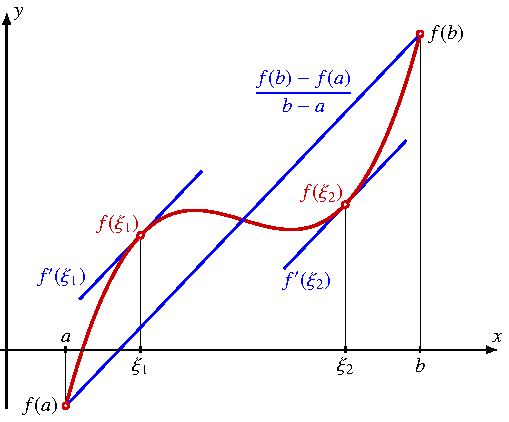
\includegraphics{chapters/020-holomorph/images/mittelwert.pdf}
\caption{Der Mittelwertsatz für eine reelle, differenzierbare Funktion
besagt, dass es zu zwei Werten $a$ und $b$ immer mindestens einen
Zwischenwert $\xi$ gibt, in dem die Steigung von $f(x)$ mit dem
der Sekantensteigung zwischen den Punkten $(a,f(a))$ und $(b,f(b))$
übereinstimmt.
\label{buch:holomorph:fig:mittelwert}}
\end{figure}
%

\begin{satz}[Mittelwertsatz]
\index{Mittelwertsatz}%
Ist $f\colon I \to \mathbb{R}$ eine stetig differenzierbare Funktion auf
dem Intervall $I=[a,b]$, dann gibt es ein $\xi \in I$ derart, dass
\[
f'(\xi)
=
\frac{f(b)-f(a)}{b-a}.
\]
\end{satz}

In dieser Form hängt er mit dem Zwischenwertsatz zusammen, der
Aussage, dass es für eine stetige Funktion $f$ für ein $\eta\in [f(a),f(b)]$
eine Stelle $\xi\in[a,b]$ geben muss, für die $f(\xi)=\eta$ ist.
So eine Aussage kann für komplexe Funktionen nur schon deshalb nicht
gelten, weil es im Komplexen keine Ordnungsrelation gibt.

Man kann den Mittelwertsatz aber auch als die Aussage sehen, dass 
die Funktionswerte an den Endpunkten des Intervalls nicht zu weit
auseinander liegen können, wenn die Ableitung klein ist.
In dieser Form gilt der Mittelwertsatz auch für Funktionen
mehrerer Variablen, braucht dazu aber das Konzept der Norm einer
linearen Abbildung.

\begin{definition}[Norm]
\index{Norm}%
Sei $A\colon \mathbb{R}^n\to\mathbb{R}^m$ eine lineare Abbildung.
Die \emph{Norm} von $A$ ist
\[
\| A\|
=
\sup_{x\in\mathbb{R}^n\setminus\{0\}} \frac{|Ax|}{|x|}.
\]
\end{definition}

Die Norm von $\|A\|$ ist auch der maximale Wert, den $|A|$ für 
Vektoren $x$ auf der Einheitskugel in $\mathbb{R}^n$ annimmt.
Der Mittelwertsatz lautet damit jetzt wie folgt.

\begin{satz}[Mittelwertsatz]
\index{Mittelwertsatz}%
Sei $U\subset \mathbb{R}^n$ ein Gebiet in $\mathbb{R}^n$ und seien
$x_0\in U$ und $x_0+t\in U$ zwei Punkte in $U$ derart, dass auch
die Verbindungsstrecke in $U$ enthalten ist.
Dann gilt
\[
|f(x_0+t) - f(x_0)|
\le
|t|\cdot \sup_{0\le \xi \le 1} \| \Jf(x_0+\xi t) \|,
\]
wobei $\Jf$ die $m\times n$-Jacobi-Matrix
\[
\Jf(x) = \frac{\partial (f_1,\dots,f_m)}{\partial(x_1,\dots,x_n)}
\]
ist.
\end{satz}

Für eine komplexe Funktion nimmt dieser Satz eine besonders einfach
Form an, weil die Ableitung von $f$ durch eine einzige komplexe
Zahl beschrieben wird.
Die Norm der Ableitung ist
\[
\| \Jf(z) \|
=
\sup_{|w|=1} | f'(z)\cdot w |
=
\sup_{|w|=1} |f'(z)| \cdot |w|
=
|f'(z)|.
\]
Die Norm ist also nichts anderes als der Betrag der komplexen 
Ableitung.
Der Mittelwertsatz für komplexe Funktionen lautet daher wie folgt.

\begin{satz}[Mittelwertsatz für holomorphe Funktionen]
\index{Mittelwertsatz}%
Sei $f$ eine in $U$ holomorphe Funktion und $z_0$ und $z_0+t$ Punkte
in $U$ derart, dass auch ihre Verbindungsstrecke in $U$ enthalten ist.
Dann gilt
\[
|f(z_0+t) - f(x_0)|
\le 
|t| \sup_{0\le \xi \le1}  |f'(z_0+\xi t)|.
\]
\end{satz}

Der Satz besagt also, dass der Abstand des Funktionswert $f(z_0+t)$
von $f(z_0)$ durch die Ableitung $f'(z)$ auf der Strecke zwischen
$z_0+t$ und $z_0$ und durch die Länge der Strecke beschränkt ist.
Er ist das zentrale Werkzeug um zu beweisen, dass die Ableitung einer
gleichmässig konvergierenden Funktionenreihe gliedweise gebildet
werden kann, wenn die abgeleitete Reihe konvergiert.
Dies wird im Abschnitt~\ref{buch:holomorph:holomorph:subsection:potenzreihen}
benötigt um zu zeigen, dass sich konvergente Potenzreihen gliedweise
ableiten lassen.

%
% Ableitung algebraischer Funktionen
%
\subsubsection{Ableitung algebraischer Funktionen}
Sei $f(z)$ eine über dem Funktionenkörper $K$ algebraische Funktion
\index{algebraische Funktion, Ableitung}
mit dem Minimalpolynom
\index{Minimalpolynom}%
\[
a(X)
=
a_n(z)X^n + a_{n-1}(z)X^{n-1}+\dots a_1(z)X + a_0(z).
\]
Dann gilt die Gleichung
\begin{equation}
a_n(z)f(z)^n
+
a_{n-1}(z)f(z)^{n-1}
+
\dots
+
a_1(z) f(z)
+
a_0(z).
\label{buch:holomorph:holomorph:eqn:algebraisch}
\end{equation}
Nehmen wir zusätzlich an, dass alle Funktionen in $K$ holomorph sind,
dann können wir 
\eqref{buch:holomorph:holomorph:eqn:algebraisch}
differenzieren.
Nach der Produkt- und der Kettenregel wird aus dem Term $a_k(z)f(z)^k$
\[
\frac{d}{dz}
a_k(z)f(z)^k
=
a_k'(z) f(z)^k
+
a_k(z)kf'(z)f(z)^{k-1}.
\]
Fassen wir in der Ableitung von
\eqref{buch:holomorph:holomorph:eqn:algebraisch}
die Terme mit und ohne $f'(z)$ zusammen, erhalten wir
\begin{align}
0
&=
a_n'(z)f(z)^n+\dots a_1'f(z)+a_0'(z)
+
\bigl(
a_n(z)nf(z)^{n-1}
+
\dots
+
a_1(z)
\bigr)
f'(z),
\notag
\intertext{die wir nach $f'(z)$ auflösen können:}
f'(z)
&=
\frac{
a_n'(z)f(z)^n+\dots a_1'f(z)+a_0'(z)
}{
a_n(z)nf(z)^{n-1}
+
\dots
+
a_1(z)
}.
\label{buch:holomorph:holomorph:eqn:ablalg}
\end{align}
Der Nenner auf der rechten Seite von
\eqref{buch:holomorph:holomorph:eqn:ablalg}
kann nicht identisch verschwinden, denn dann wäre der Nenner
ein Polynom kleineren Grades, welches die algebraische Funktion
$f(z)$ bereits definiert, im Widerspruch zur Annahme, dass $a(X)$
das Minimalpolynom war.

\begin{satz}[Ableitung algebraischer Funktionen]
\label{buch:holomorph:holomorph:satz:holoalg}
Ist $f(z)$ eine über einem Körper $K$ von holomorphen Funktionen
algebraische Funktion, dann ist $f(z)$ holomorph und die Ableitung ist
durch
\eqref{buch:holomorph:holomorph:eqn:ablalg}
gegeben.
\end{satz}

\begin{beispiel}
Die Kubikwurzel einer komplexen Zahl ist algebraisch mit dem Minimalpolynom
\index{Kubikwurzel}%
$a(X)=X^3-z$.
Nach dem Satz~\ref{buch:holomorph:holomorph:satz:holoalg} ist eine
Kubikwurzel holomorph und und nach der Formel
\eqref{buch:holomorph:holomorph:eqn:ablalg}
gilt
\[
\frac{d}{dz}
\!\sqrt[3]{z}
=
\frac{-1}{3(\!\sqrt[3]{z})^2},
\]
was der aus der reellen Analysis bekannten Formel $-\frac13z^{-\frac23}$ 
entspricht.
\end{beispiel}

